% !TEX root = ../main.tex

%************************************************
\chapter{Narrow line region properties}
\label{ch:nlr} 
%************************************************

\section{Introduction}

Correlations between the masses of super-massive black holes and properties of the host galaxy bulges in nearby galaxies \citep{gebhardt00,ferrarese00} and the similarity of the cosmic evolution of star formation and black hole activity \citep{boyle98,madau14} suggest that the formation and evolution of supermassive black holes and their host galaxies are linked. 
Active galactic nuclei (AGN) and quasar feedback, in which star formation in the host galaxy is supressed by the energy output from the quasar, is a favoured model.
This has motivated a considerable amount of observational work searching for feedback signatures \citep[for recent reviews, see][]{alexander12,fabian12,heckman14}. 

The [\ion{O}{III}]\ll4960,5008 doublet is the strongest narrow line found in optical quasar spectra.
It is forbidden line which traces gas on kiloparsec scales.  
High velocity dispersions or strong asymmetries in forbidden lines are evidence of high velocity extended ionized outflows.
Recent studies have provided constraints on the prevalence of ionized outflows traced by [\ion{O}{III}] emission in low-redshift type 2 AGN \citep[e.g.][]{mullaney13,zakamska14} using spectra from the Sloan Digital Sky Survey \citep[SDSS;][]{york00}. 
However, the signatures of feedback are expected to be stronger at higher redshifts ($z\sim2$) when the black hole accretion and star formation rates both peak. 

In this paper we analyse the [\ion{O}{III}] properties of a sample of 358 high-luminosity, redshift $1.5 < z < 4$ quasars. 
In particular, we search for signs of outflowing gas, which include assymetries and broad velocity widths. 
Recent near-IR spectroscopy of $z>1.5$ quasars often report exceptionally large [\ion{O}{III}] widths, with FWHM $>$ 1000\kms \citep[e.g.][]{netzer04,nesvadba08,kim13,brusa15,carniani15,perna15}. 
{\bf Add reference to WIISH paper}. 

To date, the focus has been extreme, rare, AGN sub-populations, e.g. highly reddened and obscured AGN (Banerji et al. 2012,2013,2014, Eisenhardt et al. 2012, Ross et al. 2014, Zakamska et al. 2016, WIISH paper).  
These populations provide insight into relatively short-lived phases in the AGN activity cycle. 
A more complete understanding of AGN-evolution and the physical link with the host galaxies requires the rare, extreme, sub-populations to be placed in the context of the AGN population as a whole. 

For a subsample where we have spectra covering the rest-frame ultra-violet line \ion{C}{IV}, we can test whether the strong outflows, inferred the blueshifting of \ion{C}{IV} relative to the systemic redshift, have any effect on the host galaxy on larger scales. 

Throughout this paper we adopt a flat $\Lambda$CDM cosmology with $h_0=0.69$ and $\Omega_M=0.29$. 

The paper is structured as follows. 

\section{Quasar Sample}

\begin{figure}
    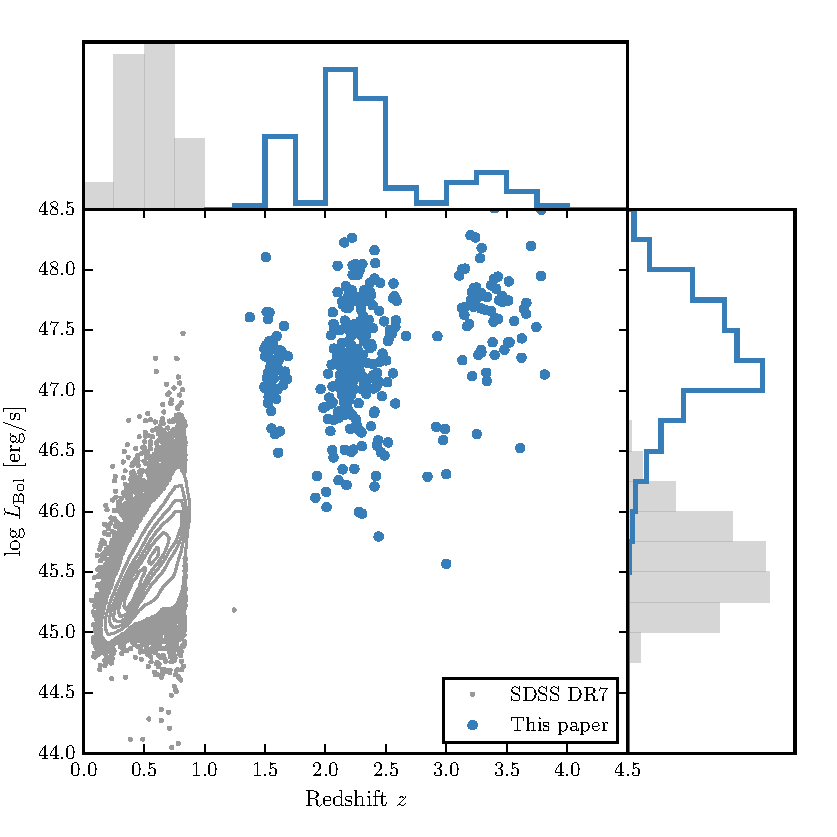
\includegraphics[width=0.8\textwidth]{figures/chapter04/luminosity_z.pdf} 
    \caption{The ranges in redshift and luminosity covered by our sample, relative to the redshift-luminosity distribution of the SDSS DR7 quasar catalogue with measured [\ion{O}{III}] line properties \citep{shen11}. The gaps in our sample coverage at $z\sim1.8$ and $z\sim3$ are due to the near-infrared transmission windows. In regions of high point-density, contours show equally-spaced lines of constant probability density generated using a Gaussian kernel-density estimator.}     
    \label{fig:lzplane}
\end{figure}

We have assembled a catalogue of 358 high-luminosity, redshift $1.5 < z < 4$ quasars, with spectra taken in the near-infrared.
At these redshifts the spectra cover the rest-frame optical region, which includes the broad Balmer \hb line and the strong, narrow [\ion{O}{III}] doublet. 
There is a significant overlap between the sample presented here and the one used in Coatman et al. (2016b), hereafter paper I.  
We briefly describe the catalogue below, but refer the reader to Coatman et al. (2016b) for further details, including the reduction procedure.  

Two hundred are selected from the SDSS Seventh Data Release \citep[DR7;][]{schneider10}. 
These are observed with LIRIS \citep{manchado98} on the William Herschel Telescope (WHT), TripleSpec \citep{wilson04} on the Astrophysics Research Consortium (ARC) 3.5\,m telescope, FIRE \citep{simcoe10} on the Magellan-Baade telescope, the SINFONI integral field spectrograph \citep{eisenhauer03,bonnet04} on the European Southern Observatory (ESO) Very Large Telescope (VLT), SOFI \citep{moorwood98a} on the New Technology Telescope (NTT), and TRIPLESPEC on the Palomar 200-inch Hale telescope (P200).
One hundred and seventeen were observed to measure accurate redshifts of quasar pairs at very close projected separations \citep{prochaska09,lau15,hennawi15}. 
Spectra were taken with GNIRS \citep{elias06} on the Gemini North telescope, ISAAC \citep{moorwood98b} on the European Southern Observatory (ESO) Very Large Telescope (VLT), NIRSPEC \citep{mclean98} on the Keck-II telescope, NIRI \citep{hodapp03} also on Gemini North, and XSHOOTER \citep{vernet11}, again, on the VLT.
Seventy-nine are bright Hamburg-ESO quasars observed with SINFONI, ninety are quasars with archival high-resolution optical spectra observed with SOFI, and four are observed with XSHOOTER and presented in the XQ-100 catalogue \citep{lopez16}.

This is the largest study of the narrow line region properties of high-$z$ quasars ever undertaken. 
The redshift and luminosity coverage of the quasars in our sample is shown in Fig.~\ref{fig:lzplane}, and the quasar sample is summarised in Table~\ref{tab:specnums}.
Our sample covers much higher redshifts and luminosities than the SDSS sample.  

\begin{table}
  \centering
  \caption{The numbers of quasars with [\ion{O}{III}] line measurements and the spectrographs and telescopes used to obtain the near-infrared spectra. Further details on the instrumental configurations are given in paper I. {\bf Check numbers.} }
  \label{tab:specnums}
    \begin{tabular}{ccc} 
    \hline
    Spectrograph & Telescope & Number \\
                 &           & \\
    \hline
    FIRE         & MAGELLAN  & 32 \\
    GNIRS        & GEMINI-N  & 29 \\
    ISAAC        & VLT       & 8 \\
    LIRIS        & WHT       & 5 \\
    NIRI         & GEMINI-N  & 29 \\
    NIRSPEC      & Keck II   & 3 \\
    SINFONI      & VLT       & 76 \\
    SOFI         & NTT       & 78 \\
    TRIPLESPEC   & ARC-3.5m  & 27 \\
    TRIPLESPEC   & P200      & 46 \\
    XSHOOTER     & VLT       & 25 \\
    \hline
    & & 144 \\
    \hline
    \end{tabular}
\end{table} 


\section{Parameteric Model Fits}

In this section we describe how we measure the [\ion{O}{III}] velocity-width and parameterize asymmeteries in the line. 
We first fit a parameteric model to the [\ion{O}{III}] emission, and the nearby \hb peak.
This step is taken soley to enhance the signal-to-noise (SNR) of the spectra and to decompose the emission from \hb and the [\ion{O}{III}] doublet. 
We then calculate non-parameteric measures of the line profile from the best-fitting model. 

Before the model can be fit, the spectra must first be transformed in to the (approximate) quasar rest-frame. 
This transformation is only for practical purposes and the emission line parameters we will go on to derive are independent of the exact redshift used. 
The redshift will later be refined using the results from the fit. 
The redshift used in this transformation is either derived from a multi-component Gaussian fit to the broad \ha emission ($\sim$ 40 per cent of our sample) or, when this is not possible, from a preliminary fit to the broad \hb emission ($\sim$ 40 per cent) or narrow [\ion{O}{III}] emission (20 per cent). 
{\bf Should say whether we use peak/median etc.}

The continuum and optical \ion{Fe}{II} emission is modelled and subtracted using a recipee that is identical to the one described in paper I. 
The following model is then fit to the spectra in the wavelength interval 4700-5100\,\AA.
The fit is done as a function of the Doppler velocity shift, and we adopt the wavelength 4862.721\AA\, (the laboratory \hb wavelength) to transform wavelengths into equivalent Doppler velocities.

\hb is modelled by two Gaussians with non-negative amplitudes and FWHM greater than 1200\kms.
A handful we fix the centroids of the two Gaussians to be the same, normally because of very low S/N or because the blue wing is below the lower wavelength limit of the spectrograph. 
Any contribution to the \hb emission from the narrow-line region is weak in the vast majority of our sample, and so we do not include an additional Gaussian component to model this emission. 
Note: we do in fact include narrow components for eight objects in our sample. 
Although, for some objects, this could bias our estimate of the velocity-width of the broad component, this information is not used in the analysis presented in this paper. 

Each component of the [\ion{O}{III}] doublet is fit with one or two Gaussians, depending on the fractional reduced $\chi^2$ difference between the one- and two-component models. 
If the addition of the second Gaussian decreases the reduced $\chi^2$ by more than 5 per cent then the double-Gaussian model is accepted.
One hundred and twenty-five are fit with a single Gaussian, 147 with two Gaussians, and [\ion{O}{III}] is undetected in a further 78 quasars.
When a single Gaussian is used to model each line, the peak flux ratio of the [\ion{O}{III}] 4960\,\AA\, and 5008\AA\, components are fixed at the expected 1:3 ratio and the width and velocity offsets are set to be equal.
In the double Gaussian fit, the peak flux ratio of the second components is again fixed at 1:3, and the width and velocity offsets are again set to be equal. 

In six quasars a significantly better fit was obtained by allowing the flux ratio between the two components to vary.
In these quasars the best-fitting peak ratio varies from 0.50 to 0.84, with mean 0.70.
{\bf Check ICA component fits to see if this looks real.}

Model parameters were derived using a standard variance-weighted least-squares minimisation procedure employing the Levenberg-Marquardt algorithm. 
Prior to the fit, the spectra were inspected visually and regions significantly affected by telluric absorption or of low S/N were masked out.

{\bf However, the fits aren't always good. How to be quantative about this? Chi-squared values indicating bad fits? Also the fact that we sometimes model Fe as OIII. Discuss the limitations of using the Boroson \& Greene template? Even if don't use results, should discuss Gaussian fits and their limitations, because that's what most people will be using.}

\begin{figure*}
    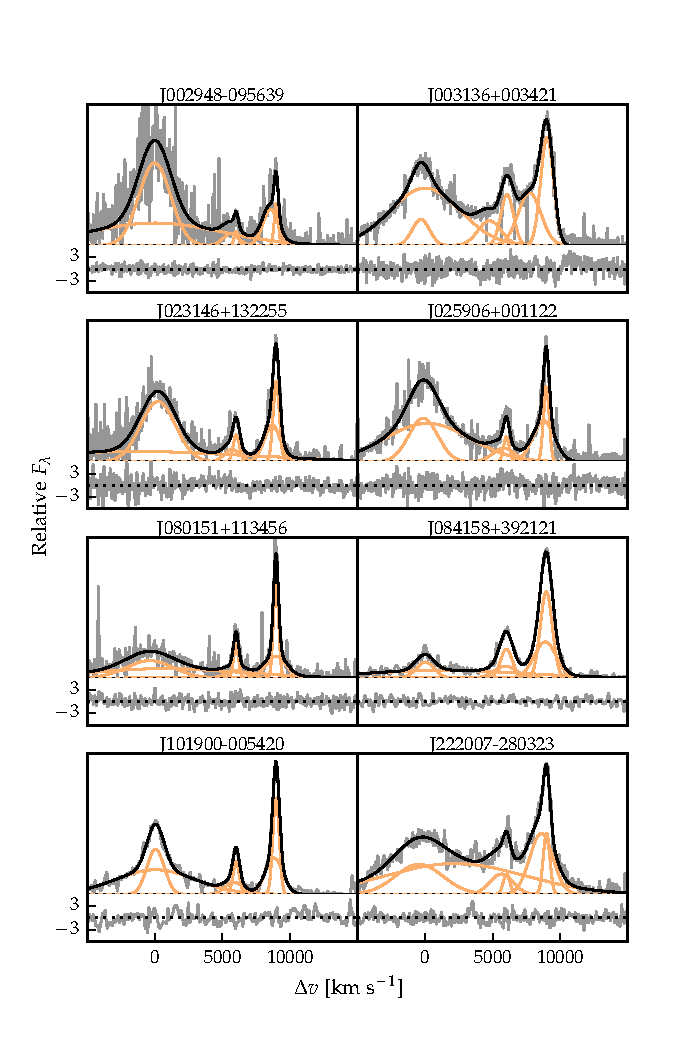
\includegraphics[width=\textwidth]{figures/chapter04/example_spectrum_grid.pdf} 
    \caption{Multi-component Gaussian fits to the continuum-subtracted \hbns/[\ion{O}{III}] emission in 16 quasars, chosen to be the representative of the wide range of [\ion{O}{III}] line widths we measure in our sample. The data is shown in grey, the best-fitting parametric model in black, and the individual model components in orange. The broad \hb centroid is used to measure the systemic redshift, and $\Delta{v}$ is the velocity shift from the line rest-frame transition wavelength for \hbns. Below each fit we plot the data minus model residuals, scaled by the errors on the fluxes. {\bf Resample model at higher resolution.}}     
    \label{fig:example_spectrum_grid}
\end{figure*}

\subsection{Derived Parameters}

\begin{figure*}
    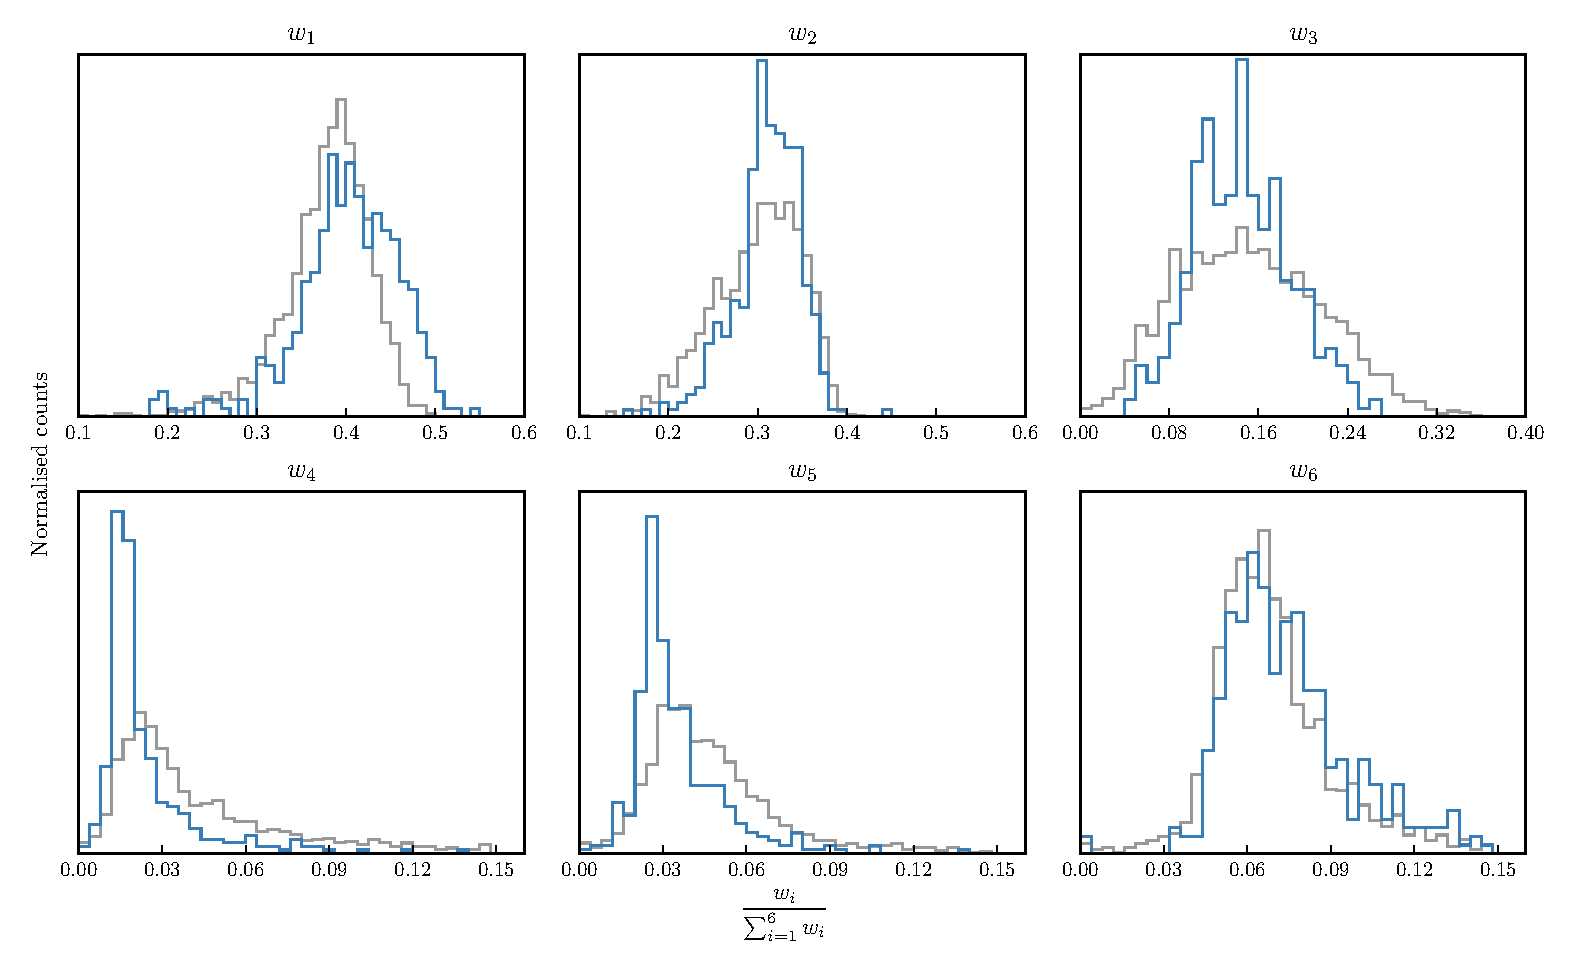
\includegraphics[width=\textwidth]{figures/chapter04/mfica_component_weights.pdf} 
    \caption{The relative weight in each of the six positive ICA components for the high-luminosity (blue) and low luminosity samples (grey). In the high-luminosity sample \ion{Fe}{II} emission is stronger (component $w_1$). The core [\ion{O}{III}] emission is weaker (components $w_4$, $w_5$) but the strength of the blueshifted wing is the same ($w_6$).}     
    \label{fig:mfica_component_weights}
\end{figure*}

\begin{figure*}
    \centering
    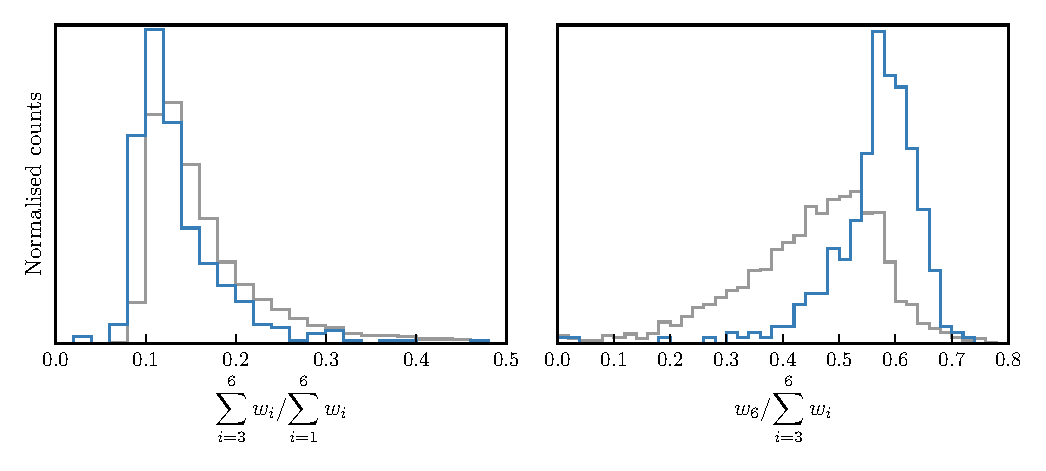
\includegraphics[width=\textwidth]{figures/chapter04/mfica_oiii_weight.pdf} 
    \caption{The relative weight in the three ICA components corresponding to [\ion{O}{III}] emission ({\em left}) and the relative weight of the component most closely related to blueshifted [\ion{O}{III}] emission relative to all three [\ion{O}{III}] components ({\em right}). [\ion{O}{III}] emission is weaker in the high-luminosity sample, but the relative contribution but the fractional contribution from the blueshifted component to the total [\ion{O}{III}] emission is higher. Hence [\ion{O}{III}] is weaker, broader, and more asymmetric in the high-luminosity sample. See Zakamska discussion.}     
    \label{fig:mfica_oiii_weight}
\end{figure*}

\begin{table}
  \centering
  \caption{Approximate physical origin of the ICA components.}
  \label{tab:icacomps}
    \begin{tabular}{cc} 
    \hline
    Component & Origin \\
    \hline
    $w_1$& \ion{Fe}{II} \\
    $w_2$& \hbns \\
    $w_3$& \hbns \\
    $w_4$& [\ion{O}{III}] core \\
    $w_5$& [\ion{O}{III}] core \\
    $w_6$& [\ion{O}{III}] wing \\
    \hline
    \end{tabular}
\end{table} 


\begin{figure}
    \centering
    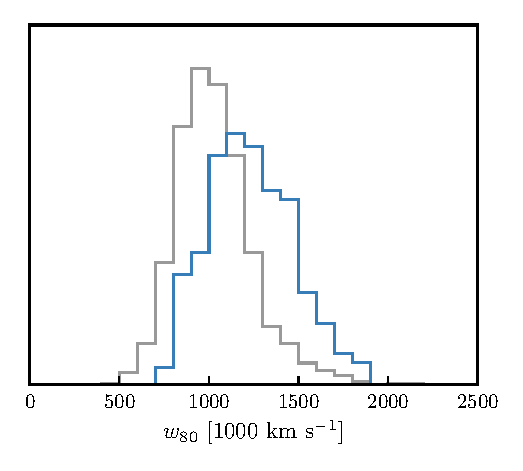
\includegraphics[width=0.6\textwidth]{figures/chapter04/mfica_oiii_w80_comparison.pdf} 
    \caption{Comparison of [\ion{O}{III}] velocity-widths in the high and low luminosity samples using the ICA component fits. If keep this need to explain in text how $w_{80}$ is calculated from ICA component fits.}
    \label{fig:mfica_oiii_w80_comparison}
\end{figure}

\begin{figure}
    \centering
    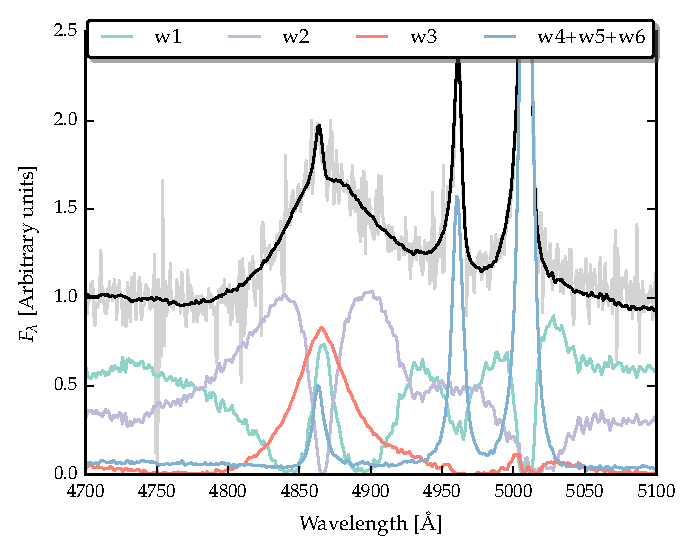
\includegraphics[width=0.6\textwidth]{figures/chapter04/mfica_components.pdf} 
    \caption{Black solid line is the median from the ICA fits to the high-luminosity sample. Black dashed line shows the median from the low-luminosity sample. The six positive ICA components are also shown.}     
    \label{fig:mfica_components}
\end{figure}

\begin{figure}
    \centering
    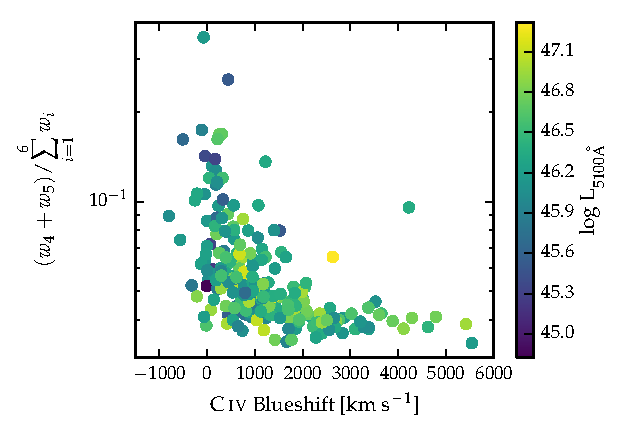
\includegraphics[width=\textwidth]{figures/chapter04/civ_blueshift_oiii_strength.pdf} 
    \caption{[\ion{O}{III}] strength decreases as the \ion{C}{IV} blueshift increases, I run in to problems comparing the \ion{C}{IV} blueshift to the [\ion{O}{III}] blueshift / velocity-width. See similar thing if I use [\ion{O}{III}] EQW instead. Need to fix y ticks. Only showing the core components here. The \ion{C}{IV} blueshift is now measured relative to the NIR ICA redshift. I think this is trend is mostly being driven by the Eigenvector 1 correlations: as the blueshift increases the \ion{Fe}{II} strength increases and the [\ion{O}{III}] strength decreases. Doesn't appear to be driven by the luminositiy. Is this tighter than EV1 trend shown with Fe/OIII strength by other authors? Is the AGN NLR absent in objects where outflows have reached
    kiloparsec scales, sweeping up the low-density material responsible for the [OIII]-emission?}     
    \label{fig:civ_blueshift_oiii_strength}
\end{figure}

\begin{figure}
    \centering
    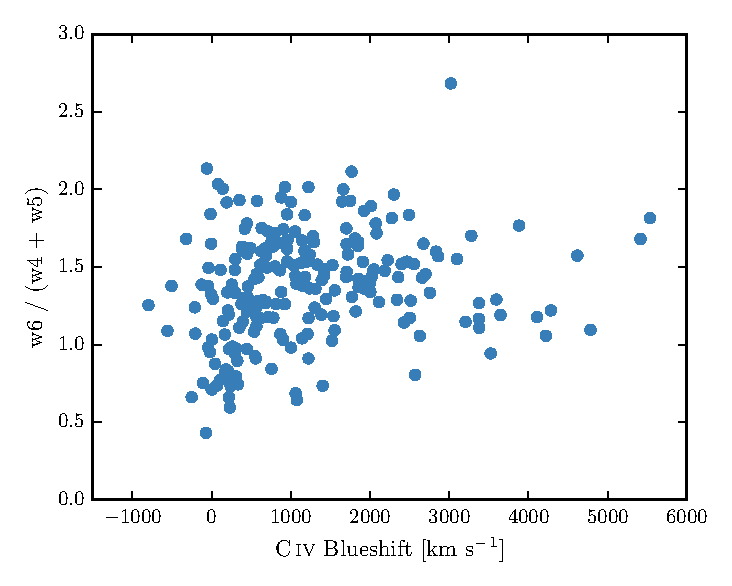
\includegraphics[width=\textwidth]{figures/chapter04/civ_blueshift_oiii_blueshift_components.pdf} 
    \caption{I think there is a trend here but at high blueshifts the OIII is undetected / very low S/N. Need to determin when we can believe OIII paramters. Why at low CIV blueshift is there a much bigger dynamic range than in [\ion{O}{III}] blueshifts in Fig. 13. Is it just because we have more objects?}     
    \label{fig:civ_blueshift_oiii_blueshift_components}
\end{figure}

\begin{figure}
    \centering
    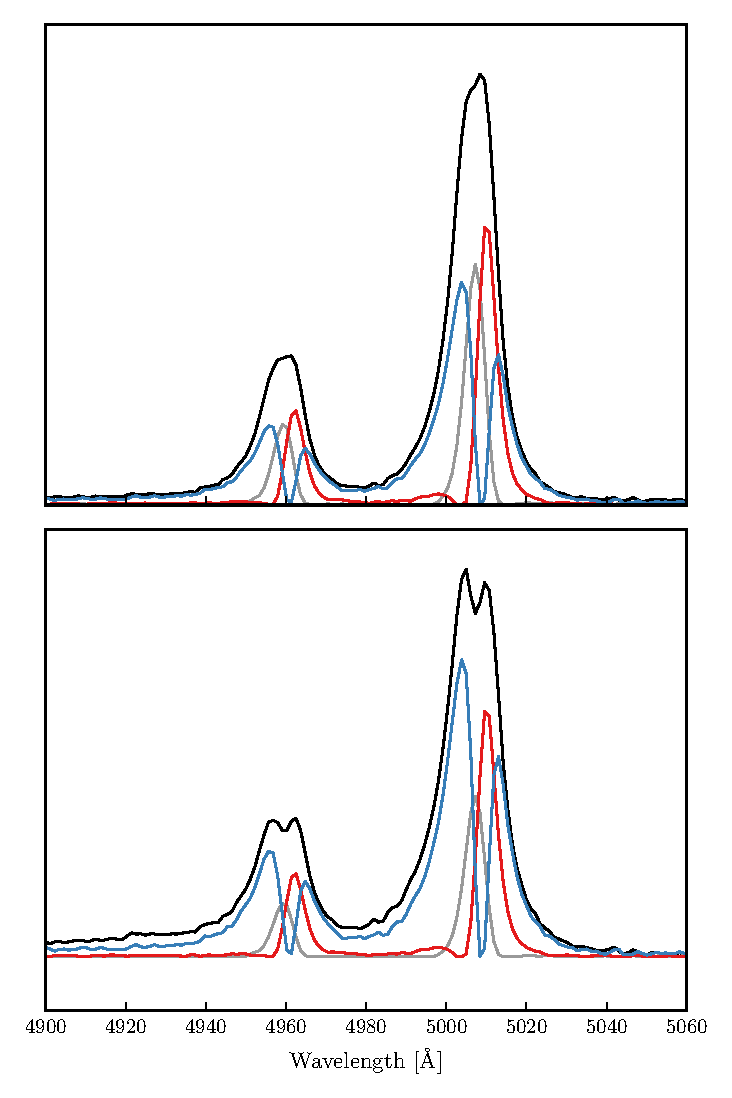
\includegraphics[width=\columnwidth]{figures/chapter04/mfica_components_oiii_comparison.pdf} 
    \caption{Comparison of median [\ion{O}{III}] profiles from ICA fits it low- and high-luminosity samples.}     
    \label{fig:mfica_components_oiii_comparison}
\end{figure}

\begin{figure}
    \centering
    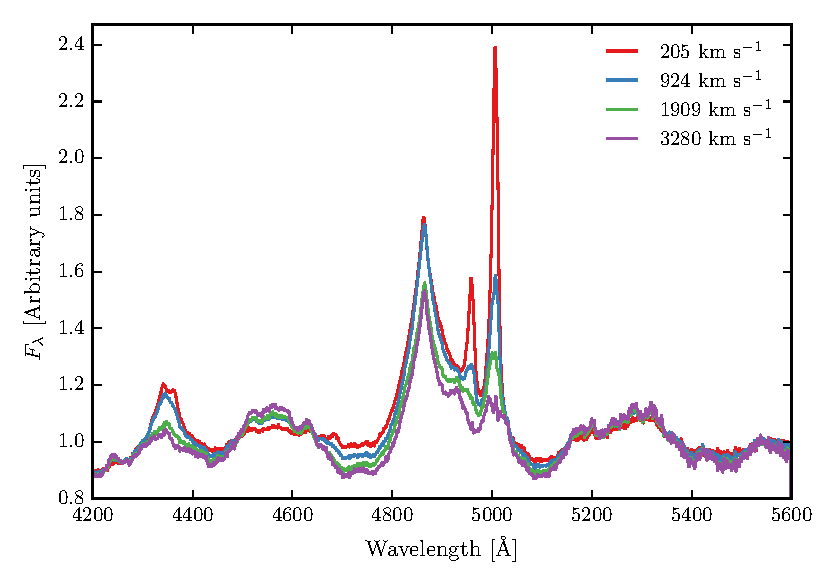
\includegraphics[width=\columnwidth]{figures/chapter04/mfica_composites.pdf} 
    \caption{ICA median weights as a functino of the CIV blueshift.}     
    \label{fig:mfica_composites}
\end{figure}

\begin{figure}
    \centering
    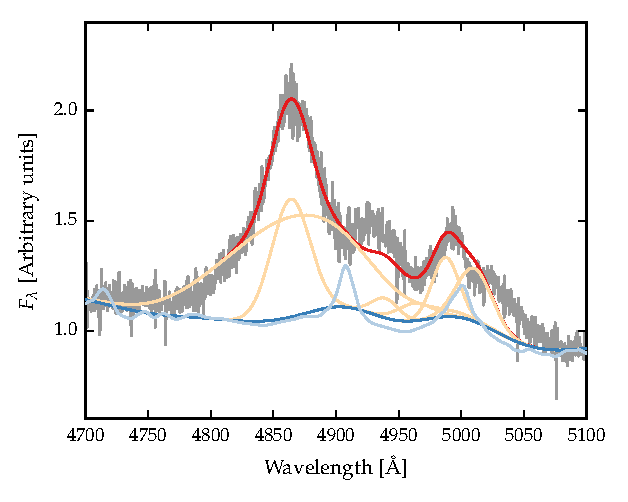
\includegraphics[width=\columnwidth]{figures/chapter04/compare_gaussian_ica_QSO538.pdf} 
    \caption{Example where poorly subtracting the iron can be confused with [\ion{O}{III}].}     
    \label{fig:compare_gaussian_ica}
\end{figure}

All [\ion{O}{III}] line properties are derived from the [\ion{O}{III}]5008 emission, but, as described below, the kinematics of the peak at 4960\AA\, are constrained by our fitting routine to be identical.

We do not to attach any physical meaning to the individual Gaussian components used in the model. 
While it is true that in some quasars the [\ion{O}{III}] emission can be clearly separated in to a narrow component at the systemic redshift and a lower-amplitude, blueshifted broad component \citep[e.g.][]{shen16a}, often this decomposition is highly uncertain.
Furthermore, often the S/N is not sufficient to statistically justify the addition of a second Gaussian component.  
Instead, we characterize the [\ion{O}{III}] line profile using a number of non-parameteric measures, which are commonly used in the literature \citep[e.g.][]{zakamska14,zakamska16}. 
A normalised cumulative velocity distibution is constructed from the best-fitting model, from which the velocities below which 5, 10, 25, 50, 75, 90, and 95 per cent of the total flux accumulates can be read off. 
The width of the emission line can then be defined, for example, using $w_{80} = v_{90} - v_{10}$. 
The absolute assymetry in the line profile $A$ is defined as $((v_{95} - v_{50}) - (v_{50} - v_{5})) / (v_{95} - v_{5})$ \citep{zakamska14}. 

We also define the blueshift of the [\ion{O}{III}] emission, which is a measure of the velocity shift of the profile from the expected position. 
This requires a measure of the observed line position, and an accurate measurement of the quasar systemic redshift. 
We use $v_{10}$ to mesaure the location of the [\ion{O}{III}] emission. 
Note that $v_{50}$ is not suitable because when [\ion{O}{III}] is low S/N we fit with single Gaussian. 

{\bf The line width measures are not at present corrected for instrumental broadening, but this can easily be done.}

\begin{figure}
    \centering
    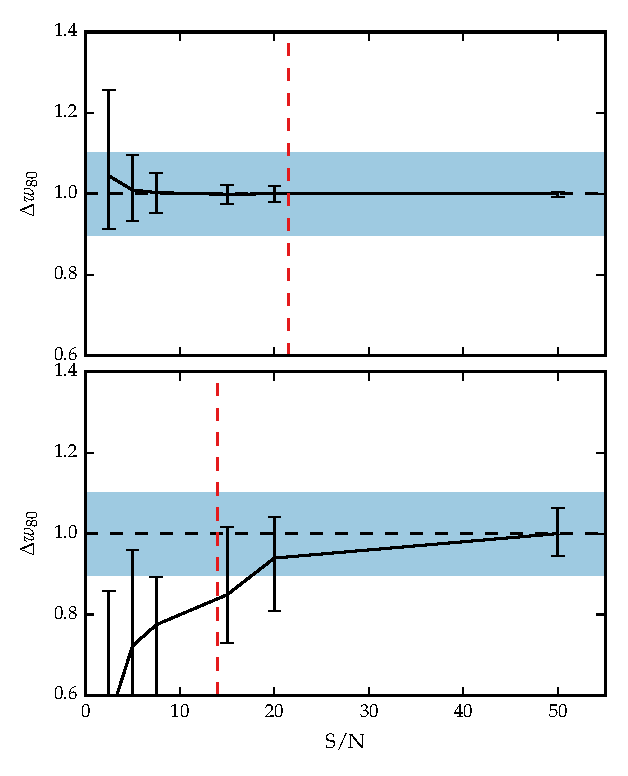
\includegraphics[width=\columnwidth]{figures/chapter04/snr_test.pdf} 
    \caption{}
    \label{fig:snr_test}
\end{figure}


\subsection{Other flags}

\subsubsection{Flag 2}

Low S/N. Includes some of the strong iron emitters. 


\subsubsection{Flag 3}

74 objects where [\ion{O}{III}] is undetected, although I don't have a rigorous definition of what this means. 
Merge with 2? 


\section{ICA Component Fits}

What is the segue here? 
Sometimes Gaussians give poor fit? Not clear what is Hb, what is OIII, what is Fe? Show some examples of when the multi-Gaussian fits fail. 
Need to describe sample used in ICA component decomposition and briefly describe method (or refer to Allen \& Hewett). 


\section{Measuring the quasar systemic redshift}


\begin{figure}
    \centering
    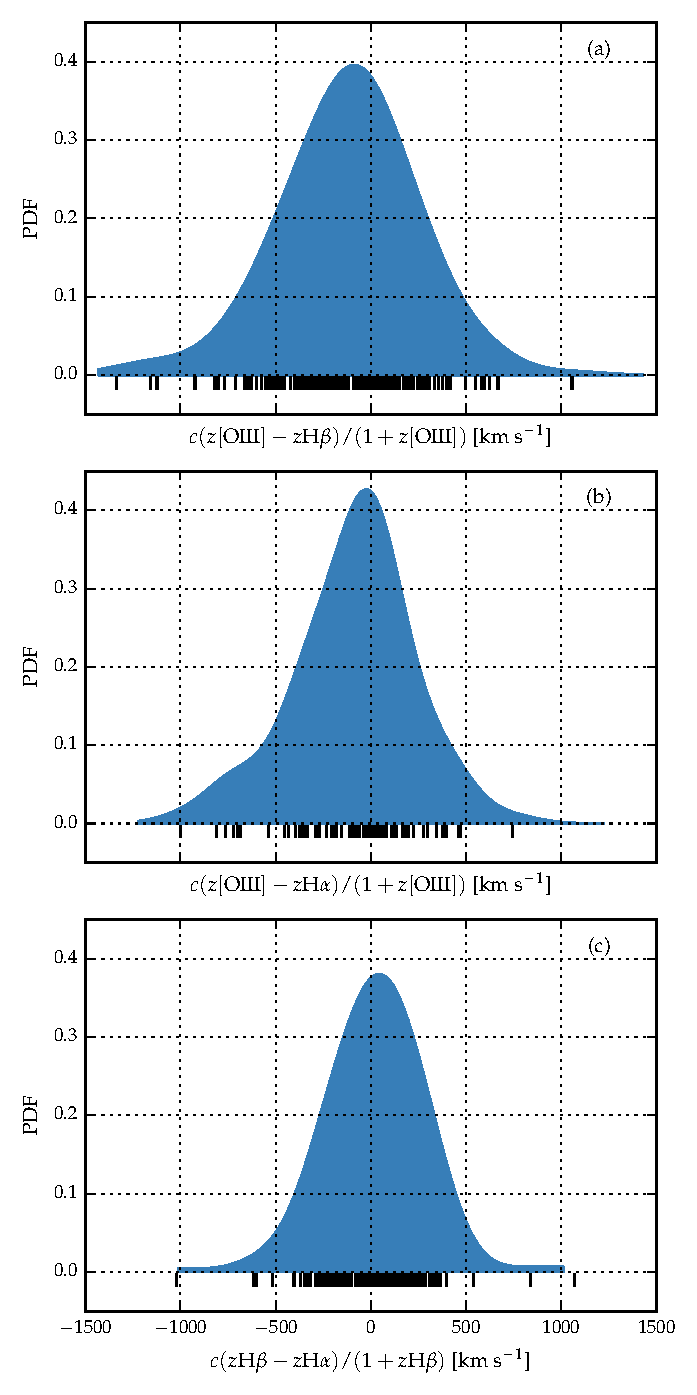
\includegraphics[width=0.8\linewidth]{figures/chapter04/redshift_comparison.pdf} 
    \caption{Redshift comparisons. Lots have been excluded from Ha/Hb so need to look at flags greater than one. What is the big peak? Gaussian fit to the first one has failed. Find out why these plots look different to ones in paper.}       
    \label{fig:redshift_comparison}
\end{figure}

Explain flags 
Need to send paul redshifts 

\subsection{\hans}

There are 224 quasars in our sample with spectra covering the \ha emission line. 
We discard seven of these from our sample because of very low S/N ($<$2.5 measured in the \ha line), leaving 217
To measure the position of the line we fit a parameteric model, which is very similar to the model described in Paper I. 
The continuum emission is first modeled and subtracted using the procedure described in Paper I. 
We then test five different models with increasing degrees of freedom to model the \ha emission. 
The model we select is the simplest model for which the fractional change in the reduced chi-squared from the model with the lowest reduced chi-squared is less than ten per cent. 

The models we test are: (1) a single broad Gaussian; (2) two broad Gaussians with identical velocity centroids; (3) two broad Gaussians with different velocity centroids; (4) two broad Gaussians with identical velocity centroids, and additional narrower Gaussians to model the narrow \ha emission, and the narrow components of [\ion{N}{II}]\ll6548,6584 and [\ion{S}{II}]\ll6717,6731; (5) two broad Gaussians with different velocity centroids, and additional narrower Gaussians. 
If used, the width and velocity of all narrow components are set to be equal in the fit, and the relative flux ratio of the two [\ion{N}{II}] components is fixed at the expected value of 2.96.
The number of quasars fit by each model is: model 1 - 10; model 2 - 71; model 3 - 32; model 4 - 51; model 5 - 53. 
The redshift is then measured at the peak flux of the \ha model, including both the broad and narrow components of \ha if appropriate. 

\subsection{ICA}

The only sensible way to measure the systemic redshift is using the NIR ICA fit. 
\ha and \hb seem to give no systematic offset but large scatter, and they are often asymmetric, so should only use peak. 
And \ha isn't always available, and have other narrow components need to decompose.
\ion{O}{III} peak is mostly fine to use, but then there are some objects where the whole line is blueshifted. 
And critically, at large CIV blueshifts the [\ion{O}{III}] emission is often undetected. 
Can show comparison of NIR ICA redshifts to... Optical ICA? Hewett \& Wild? 

Should emphasise that most people use [\ion{O}{III}] to get the most reliable systemic redshift. 
While this is fine at low luminosities, at high luminosities this can result in large errors (profile can be dominated by blueshifted component, Fe emission can be improperly subtracted, or [\ion{O}{III}] might not be detected at all. 
Publish ICA components with this paper? 

Can also describe what I found trying to get redshifts from broad \hans, \hbns? (Narrow components generally very weak at these luminosities so can't be used.)
Generally find no systematic errors but large ($\sim$1000\kms\, scatter).
Comparing NIR ICA to [\ion{O}{III}] for the [\ion{O}{III}] with high S/N I find small (few hundred \kms) scatter. 

Should publish [\ion{O}{III}] redshifts with this paper for people to use. 
 

\subsection{Parameter uncertainties and upper limits}

Describe how uncertainties on best-fitting parameters were calculated. 

In 78 quasars, or approximately 25 per cent of or sample, the [\ion{O}{III}] is undetected, or detected with very low S/N. 
In this section we describe how upper limits on the [\ion{O}{III}] equivalent width were calculated. 
Firstly, the best-fitting model comprising the continuum, \ion{Fe}{II}, and \hb emission is subtracted from the spectra, leaving behind only emission due to [\ion{O}{III}]. 
From this spectra we generate 100 mock spectra, where the flux at each wavelength is randomly drawn from a Normal distribution with a mean equal to the flux convolved with a Gaussian of width 200\kms and a width equal to the known error. 
We then perform an error-weighted linear least-squares regression with an [\ion{O}{III}] template derived from a fit to a very high S/N low redshift SDSS composite spectra. 
The equivalent width of the best-fitting model is recorded for each of the 100 realisations of the spectra. 
The error in the equivalent width is defined as the root-mean-square of these values.

Calculated uncertainties using Monte Carlo. 
Uncertainties on v10 are very large, which I think makes sense since the wing Gaussian will be appearing and disappering, giving a large dispersion in v10. Or regardles v10 is just very sensitive to the noise. 
Maybe I should be using v25 instead? 

\subsection{Absolute flux calibration of spectra and continuum luminosities}

Relative flux-calibration of the infrared spectra as a function of wavelength has been achieved, to $\simeq$10 per cent, through observations of appropriate flux standards. 
The absolute flux levels, however, can be in error by large factors due to variable atmospheric conditions combined with the narrow slit widths. 
For the majority of the quasars we have, therefore, established the absolute flux scale for each near-infrared spectrum using the same quasar SED-model fitting scheme employed in Paper I.
Briefly, the SED-model was fit, with the normalisation and E(B-V) as free varibales, to optical/infrared magnitudes, or SDSS/BOSS spectra (check order I do this.)
This allows us to extrapolate from the optical when we do not have photometric data in the near-infrared. 
The spectra were then normalised to the SED model using a linear error-weighted least-squares regression in the the regions of the spectra covered by the $H$/$K$ bands. 
The monochromatic continuum luminosity at 5100\AA was calculated directly from the normalised SED-model. 
{\bf If this sounds strange can also calculate from fit to normaised spectra.}
{\bf Check if any missing normalisation / monochromatic luminosities.} 

\section{Results from ICA fits}

Need to convince the reader that the ICA components approximately correspond to real components. 
Explain how non-parameteric measures derived form ICA reconstructions. 

We find there is a decreasing symmetric component at high luminosities. 
Relates directly to \citet{shen14}. 
A stable narrow line region is removed by the outflowing material. 
\citet{shen14} showed that the strength of the core [\ion{O}{III}] component decreases with quasar luminosity and optical \ion{Fe}{II} strength faster than the wing component, leading to overall broader and more blueshifted profiles as luminoisty and \ion{Fe}{II} strength (or \ion{C}{IV} blueshift) increases. 

\section{Luminosity/redshift-evolution of [\ion{O}{III}] properties}

\begin{figure}
    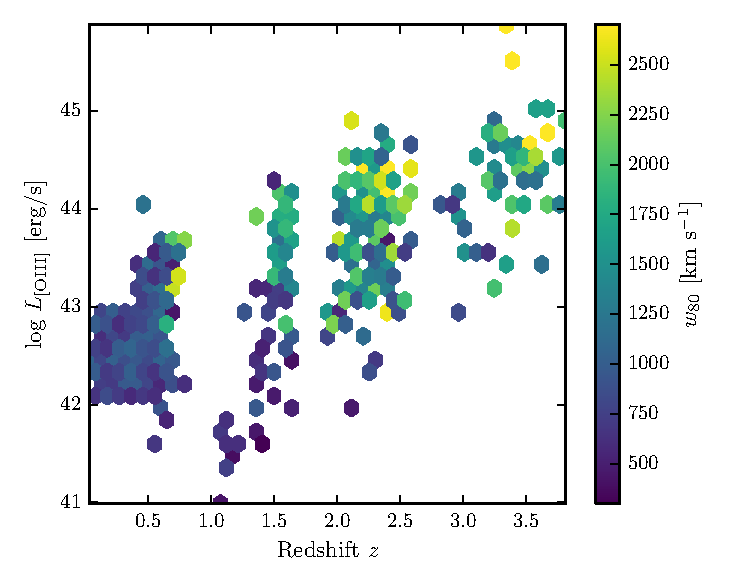
\includegraphics[width=\columnwidth]{figures/chapter04/oiii_luminosity_z_w80.pdf} 
    \caption{The [\ion{O}{III}] velocity-width, characterised by $w_{80}$, as a function the [\ion{O}{III}] luminosity and the quasar redshift. The color of each hexagon denotes the mean $w_{80}$ for the obects in that luminosity-redshift bin. We have suplemented our sample with low-$z$ objects from \citet{zakamska14} and medium ($z\sim$1.5) redshift objects from \citet{harrison16}. If I keep this plot make sure its clear which points belong to which sample.}       
    \label{fig:oiii_luminosity_z_w80}
\end{figure}

In this section we look for any luminosity/redshift dependent changes in the [\ion{O}{III}] line properties. 
To do this we extend the dynamic range of our samples in terms of both luminosity and redshift by supplementing our sample with quasars presented by \citet{zakamska14} and \citet{harrison16}. 

The \citet{zakamska14} objects are a sample of 568 obscured luminous quasars selected from SDSS \citep{reyes08,yuan16}. 
They are selected to have [\ion{O}{III}] luminosities above $10^{8.5}{\rm L}\odot$ and have a median redshift $z=0.397$. 

We also include 40 quasars at redshifts $1.1 \leq z \leq 1.7$) from the KMOS AGN Survey at High redshift (KASH$z$) with [\ion{O}{III}] line measurements. 

We also have the same information for $\sim$20\,000 SDSS spectra from \citet{mullaney13}. 

In Figure~\ref{fig:oiii_luminosity_z_w80} we show the [\ion{O}{III}] velocity width as a function of the [\ion{O}{III}] luminosity and the quasar redshift. 
The lack of any redshift-evolution between $z=0$ and $z=1.5$ was reported by \citet{harrison16}.
Our additional data suggets that this continues to $z\sim2.5$. 
On the other hand, at fixed redshift, we see a significant correlation between the [\ion{O}{III}] velocity width and the luminosity. 

The fact that we don't see many broad lines in the \citet{zakamska14} objects even at luminosities $>$43 erg/s could be due to the fact that these are all type II quasars, whereas the sample presented in this paper are all type I. 
\citet{mullaney13} showed that the [\ion{O}{III}] lines of type I quasars are typically broader than in type II quasars. 

Looking at the [\ion{O}{III}] velocity width as a function of luminosity tells us about the physical drivers of the outflows observed in [\ion{O}{III}]. 
The correlation with luminosity suggests that the highest velocity outflows are associated with the most luminous AGN. 
This has been reported for low-redshift AGN, for both ionized and molecular outflows (e.g. Westmoquette et al. 2012; Veilleux et al. 2013; Arribas et al. 2014; Cicone et al. 2014; Hill \& Zakamska 2014).

This suggests that the outflows are driven by radiative forces. 
On the other hand, \citet{mullaney13} find that once the correlation between the [\ion{O}{III}] luminosity and the radio luminosity has been taken in to account, the [\ion{O}{III}] velocity width is more strongly related to the radio luminosity of the AGN. 

\section{Equivalent width}

\begin{figure}
    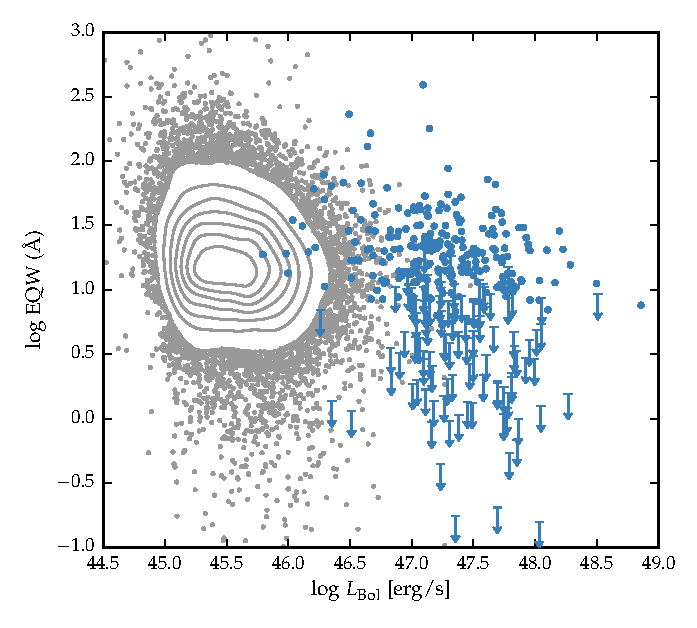
\includegraphics[width=\columnwidth]{figures/chapter04/eqw_lum.pdf} 
    \caption{The [\ion{O}{III}] EW as a function of the quasar bolometric luminosity for the sample presented in this paper (blue circles) and the low-$z$ SDSS sample (grey points and contours). Upper limits are denoted by the downward arrows.}     
    \label{fig:eqw_lum}
\end{figure}

In Fig.~\ref{fig:eqw_lum} we show the [\ion{O}{III}]5008 EW as a function of the quasar bolometric luminosity. 
Bolometric luminosity is estimated from the monochromatic continuum luminoisty at 5100\AA using the correction factor given by \citet{richards06}. 
For comparison, we also show the low-$z$ sample from \citet{shen11}.  

The equivalent width of [\ion{O}{III}] has been found to strongly decrease as a function of redshift and/or luminosity \citep[e.g.][]{brotherton96,netzer04,sulentic04,baskin05b}. 

The size of the narrow line region is roughly expected to scale as $L^{0.5}$ \citep[e.g.][]{netzer04}. 
However, for high luminosity quasars with strong [\ion{O}{III}] this gives NLR sizes which are unreasonably large \citep[$\sim$100 kpc;][]{netzer04}. 

\citet{netzer04} found 1/3 of their high luminosity sample had very weak [\ion{O}{III}], whereas quasars with weak [\ion{O}{III}] are very rare for nearby AGN. 
We find a very similar fraction. 
\citet{netzer04} claim that for the population of strong [\ion{O}{III}] emitters there is no reduction of EW with increasing source luminosity. 
On the other hand, there are many weak or no [\ion{O}{III}] emitters at high luminosity that could give the impression that the line EQW decreases with increasing source luminoisity. 

\subsection{OIII outflows}

\begin{figure}
    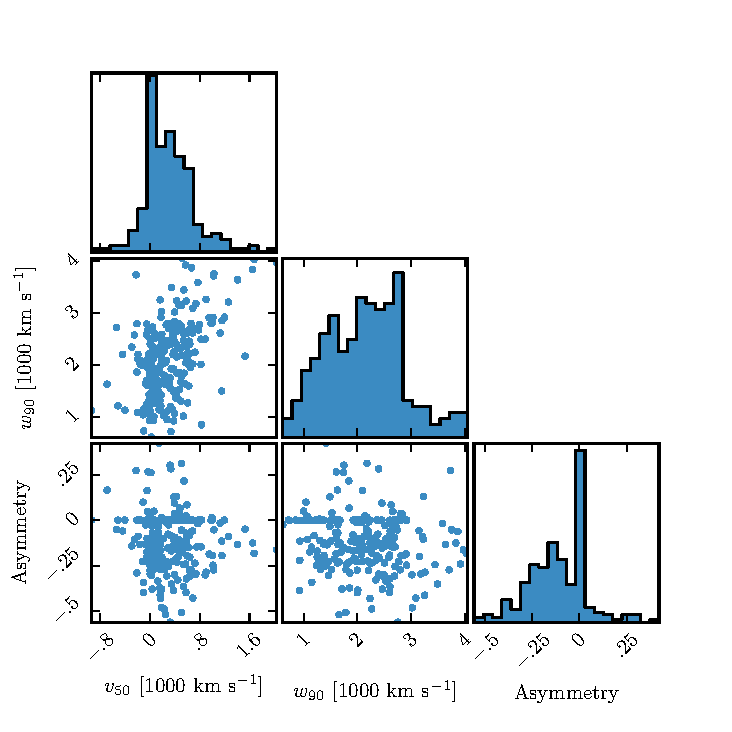
\includegraphics[width=\columnwidth]{figures/chapter04/parameters_grid.pdf} 
    \caption{The distributions of and correlations between a subset of the non-parameteric measures we made of the best-fitting [\ion{O}{III}] models.}     
    \label{fig:parameters_grid}
\end{figure}

Our best-fitting profiles show a strongly blue-asymmetric profile (Fig.~\ref{fig:parameters_grid}), with a significant fraction of the total emission in a blue wing.
The luminous blueshifted broad wing and the exteremely broad profile reveals high-velocity outflowing ionized gas. 
This can be explained if the far-side of any outflowing gas, that is moving away from the line of sight, is obscured by dust in the host galaxies (e.g. Heckman et al. 1981; Vrtilek 1985). 
Observations at both low and high redshifts commonly observe this blueshifted component.  
Our results, and those of other authors, suggest that kpc-scale outflows in ionized gas are common among the most luminous high-redshift actively accreting SMBHs.

The situtation is very different in nearby AGN, where the [\ion{O}{III}] velocity width is dominated by the galactic potential and correlates well with the stellar velocity dispersion.
HI, CO and absorption line mesaures of the host galaxy rest frame suggest that [\ion{O}{III}] usually gives consistent results within 200 km/s (de Robertis 1985; Whittle 1985; Wilson \& Heckman 1985; Condon et al. 1985; Stripe 1990; Alloin et al. 1992; Evans et al. 2001).  

We see a correlation between the [\ion{O}{III}] velocity width and blueshift. 
As the blueshift of the line increases it gets broader. 
This is consistent with \citet{shen14}, where the strength of the narrow core is decreasing, leading to a broader and more blueshifted profile. 


\subsection{[\ion{O}{III}] and \ion{C}{IV} outflows are linked}

\begin{figure}
    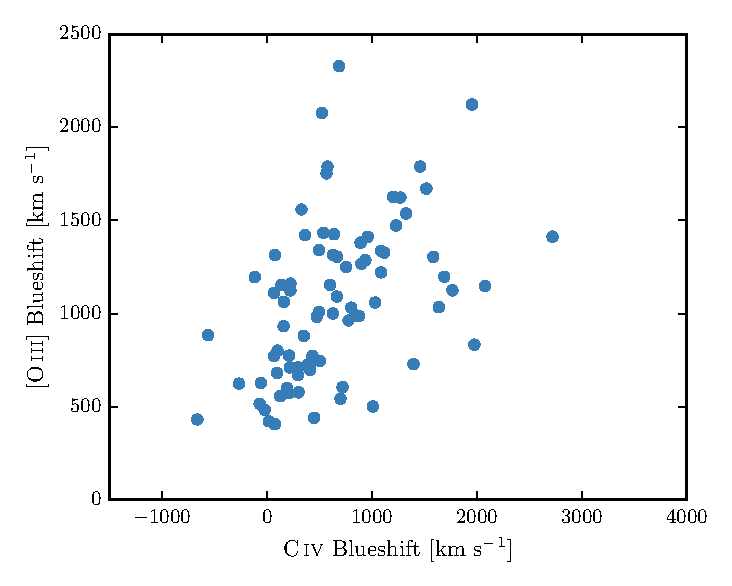
\includegraphics[width=\columnwidth]{figures/chapter04/oiii_civ_blueshifts.pdf} 
    \caption{The relation between the blueshifts of \ion{C}{IV} and [\ion{O}{III}]. Equivalent to Fig 8. We use the \hb peak in this figure, which I think is responsible for some of the trend. However, we do see a correlation (albeit noisier) using the NIR ICA redshifts. Not a sensible to use the [\ion{O}{III}] redshifts, since these become much more unreliable at the high \ion{C}{IV} blueshift end (when [\ion{O}{III}] is weaker: figure 7. Note that we are using $v_{10}$ for the [\ion{O}{III}] position and $v_{50}$ for the \ion{C}{IV} position. We can't use $v_{50}$ for [\ion{O}{III}] because sometimes we are using a single Gaussian, especially if the [\ion{O}{III}] is weaker and we miss the broad component. Need to remake this plot / don't use at all because I don't believe some of the Gaussian fits to [\ion{O}{III}], especially at high \ion{C}{IV} blueshifts when [\ion{O}{III}] is weak and \ion{Fe}{II} is strong.) Only objects where fit with two components.}     
    \label{fig:oiii_civ_blueshifts}
\end{figure}

\begin{figure}
    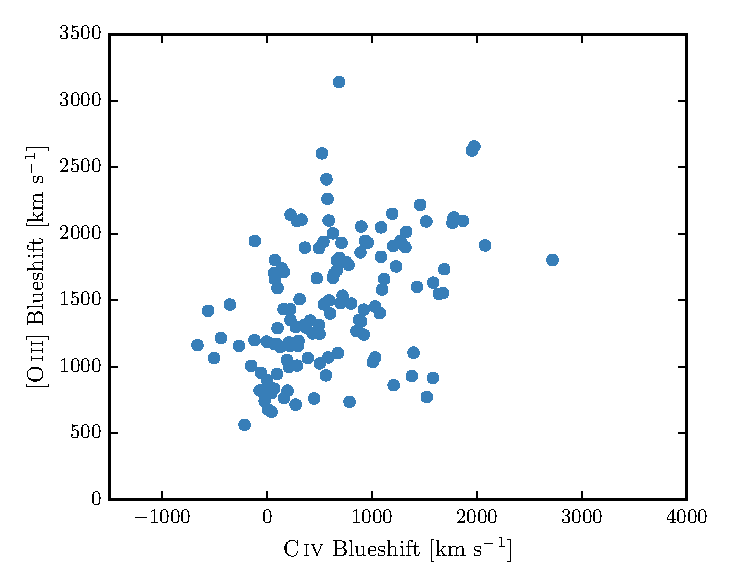
\includegraphics[width=\columnwidth]{figures/chapter04/oiii_width_civ_blueshift.pdf} 
    \caption{}     
    \label{fig:oiii_width_civ_blueshift}
\end{figure}

As described in Paper I, we have searched for optical counterparts to our near-infrared spectra. 
Optical spectra are available for XXX quasars in our catalogue, and cover the broad \ion{C}{IV} doublet. 
As we described in Paper I and \citet{coatman16}, \ion{C}{IV} is often blueshifted, which almost certainly signal the presence of strong outflows, most likely originating in a disc wind.
In Paper I we demonstrated that the quasars in our sample cover the full range of \ion{C}{IV} blueshifts seen in the SDSS quasar population, which makes our sample unique in that it allows us to study properties of the quasar across the full parameter range. 

The \ion{C}{IV} velocity centroid measurements are taken directly from paper I. 
We define the `location' of the [\ion{O}{III}] emission using $v_{10}$, although the results are the same if $v_{20}$, $v_{50}$ etc. are used instead.

In Figure~\ref{fig:oiii_civ_blueshifts} we show the \ion{C}{IV} blueshifts against the [\ion{O}{III}] blueshifts.
This comparison is done for a sub-sample of 146 objects where we have good measurements of the \ion{C}{IV}, [\ion{O}{III}], and \hb (to measure the systemic redshift) profiles. 
Objects with S/N > 3 are shown as blue filled circles and objects with S/N < 3 as open grey circles. 
We calculated the median S/N per pixel in the best-fitting model for the [\ion{O}{III}]5008 emission.

There is a clear and strong correlation. 
Similar correlations have been tentatively found in lower redshift quasars and AGN \citep{zamanov02}. 

% \begin{figure}
%     \includegraphics[width=\columnwidth]{oiii_civ_blueshifts_luminosity.pdf} 
%     \caption{Same as Fig.~\ref{fig:oiii_civ_blueshifts}, except including only high S/N points, and the colour of each point corresponds to the monochromatic continuum luminosity at 5100\AA\, of that quasar.}     
%     \label{fig:oiii_civ_blueshifts_luminosity}
% \end{figure}

The blueshifting of \ion{C}{IV} is known to correlate with luminosity \citep{richards11}.
In [\ion{O}{III}], the blueshifted wing becomes relatively more prominent as the luminosity of the quasar increases \citep{shen14}. 
Therefore, it is plausible that the correlation between the \ion{C}{IV} and [\ion{O}{III}] blueshifts is a secondary effect that is driven by the correlation of each with the luminosity. 
In Figure~\ref{fig:oiii_civ_blueshifts_luminosity} we color the data points by the luminosity, and no luminosity-dependent trends are apparent. 
We find that both the [\ion{O}{III}] and \ion{C}{IV} blueshifts are correlated with the luminosity, but that these correlations are much weaker than the correlation between the [\ion{O}{III}] and \ion{C}{IV} blueshifts. 



\section{Eigenvector one correlations}

\begin{figure}
    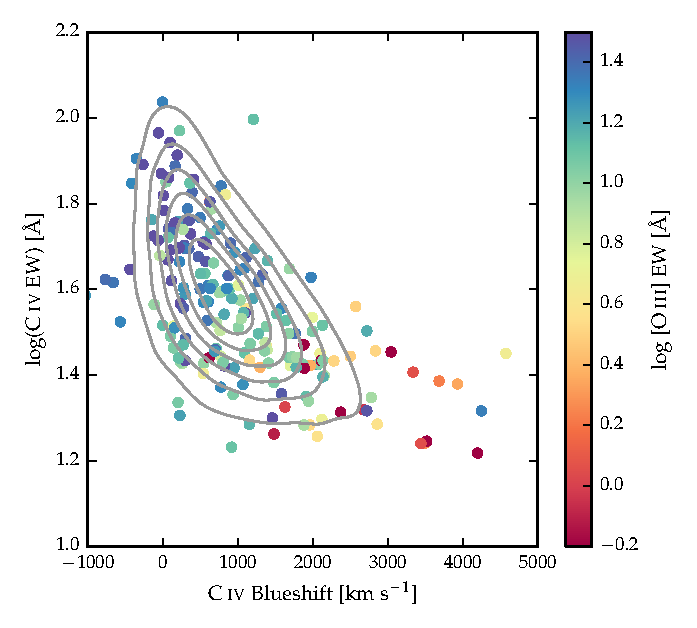
\includegraphics[width=\columnwidth]{figures/chapter04/ev1.pdf} 
    \caption{The [\ion{O}{III}] EQW as a function of the \hb FWHM and the optical \ion{Fe}{II} strength (EQW \ion{Fe}{II}/ EQW \hb).}     
    \label{fig:ev1}
\end{figure}

In Figure~\ref{fig:ev1} we show the [\ion{O}{III}] EQW as a function of the \hb FWHM and the optical \ion{Fe}{II} strength. 
The optical \ion{Fe}{II} strength is defined as the ratio of the \ion{Fe}{II} and \hb EQW, where the \ion{Fe}{II} EQW is measured between 4434 and 4684\AA.
These parameters form part of `eigenvector 1' (EV1), the first eigenvector in a principal component analysis which originated from the work of \citet{boroson92}.
In our sample, these parameters follow very similar correlations to what is observed at low-$z$ \citep[e.g.][]{shen14}.
In particular, the anti-correlation between the [\ion{O}{III}] and \ion{Fe}{II} EQWs.  

Same as \citet{shen16a}, we confirm that the EV1 correlations hold at high luminosities/redshifts. 
See also Sulentic et al. 2004, 2006; Runnoe et al. 2013. 
Make sure it's clear that \citet{shen16a} quasars make up a significant chunk of our sample. 

\section{Mapping EV1 to CIV blueshift and EQW}


\section{Signal to noise tests}


\section{Broad Absorption Line Quasars}

\begin{figure}
    \centering
    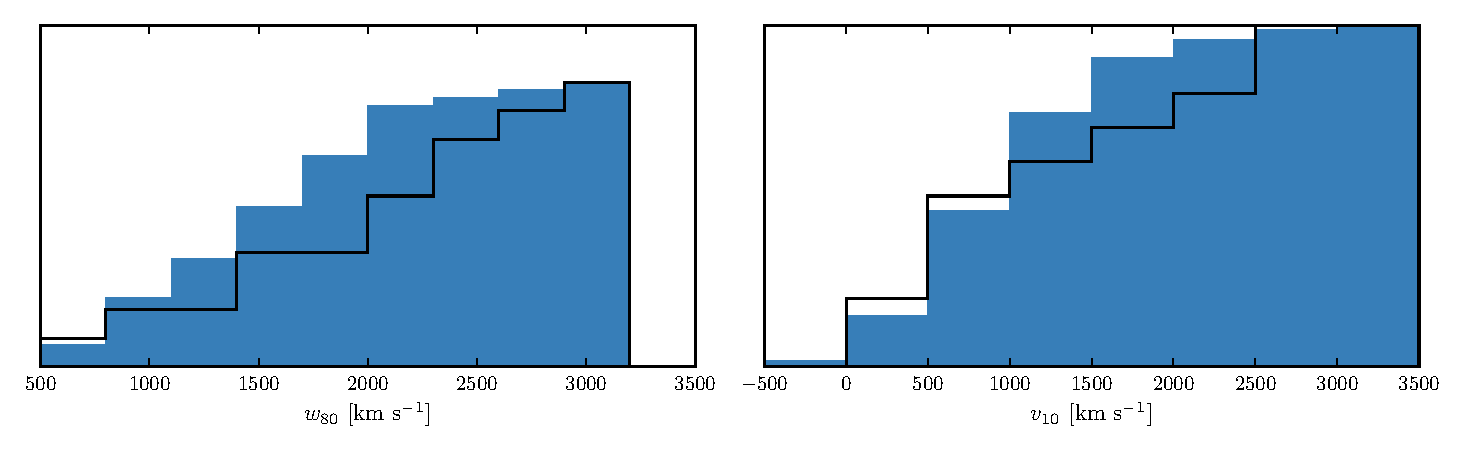
\includegraphics[width=0.8\linewidth]{figures/chapter04/bal_hists.pdf} 
    \caption{The distribution of $w_{80}$ and $v_{10}$ for the 19 BALs are compared to the distribution for the non-BALs. These look rubbish. Cumulative distributions instead? Try doing gaussian kernel density estimator}     
    \label{fig:bal_hists}
\end{figure}

19 quasars in our catalogue are classified as broad absorption line (BAL) quasars, using the either the SDSS classification flags or the \citet{allen11} catalogue. 
We find that the BAL quasars have typically broader [\ion{O}{III}] than the rest of the sample. 
Note that in the \citet{zakamska16} sample of very red quasars, the incidence of BALs is very high, and these objects have extremely broad [\ion{O}{III}] profiles. 
A two-sided Kolmogorov-Smirnov statistic on the $w_{80}$ distributions returned a p-value of 0.10. 
What does this mean?
Try with different parameters?
Histograms look rubbish so maybe just give the numbers. 

\section{Discussion}

\subsection{Type II quasars}

Implications of our findings on searches for high-redshift type 2 quasars. It could be that type II quasars exist. If you look at CIV/MgII the narrow line components are very weak. So the contribution from the narrow line region is very weak in luminous quasars, and you just won't see it even if the broad line region is obscured.
Findings in this paper seem to suggest that the startic narrow line region is very weak in luminous quasars. 